\section{Results}
We have initially evaluated the fidelity for different $ n $ for a fixed trapping $ \omega $ and we progressively increased the initial speed $ k_{0} $ until a consistent drop in fidelity was met.
We can clearly see that the curve $ \Ga_{2} $ provides the higher level of fidelity for each different $ \omega $ and it is hence preferrable.
In addition, we note that the spectrum of velocities upon which the protocol is reliable gets wider as the strength of the transverse confinment increases, as predictable.
We then decided to compare the probability density of each wave packet in the straight end after the bent section to assess the deformation of the wave function due to the bending of the waveguide, as opposed to the ideal one and once again we could see how the mixing between transverse and longitudinal components is lower for $ n = 2 $ and that is reflected in a higher level of fidelity.
\begin{figure*}[t!]
	\centering
	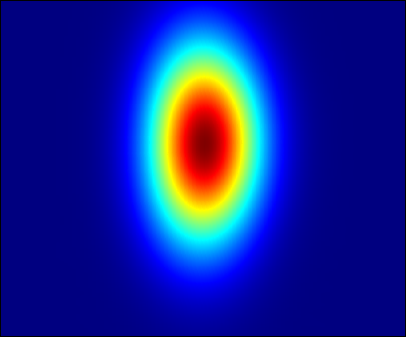
\includegraphics[width = .3\textwidth]{gfx/texdens_ord2_300_7.pdf}
	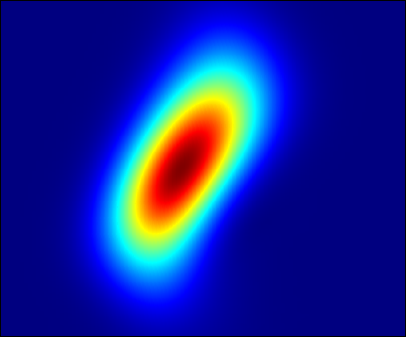
\includegraphics[width = .3\textwidth]{gfx/texdens_ord0_300_7.pdf}
	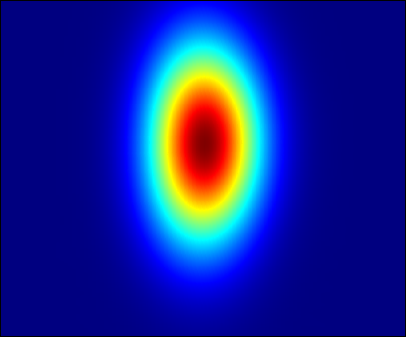
\includegraphics[width = .3\textwidth]{gfx/texdens_ord2_300_7.pdf}
	\caption{arison between the wave function density for different orders 1 to 4 (fig. (a) to (d) for $ \omega T = 7 $ and $ k_{0}R = 1100 $ with the corresponding fidelity. In fig.(a) the the mixing of the two components is more visible than the others and it is reflected in the value of the fidelity}
	\label{fig:densities}	
\end{figure*}
\begin{figure*}[t!]
		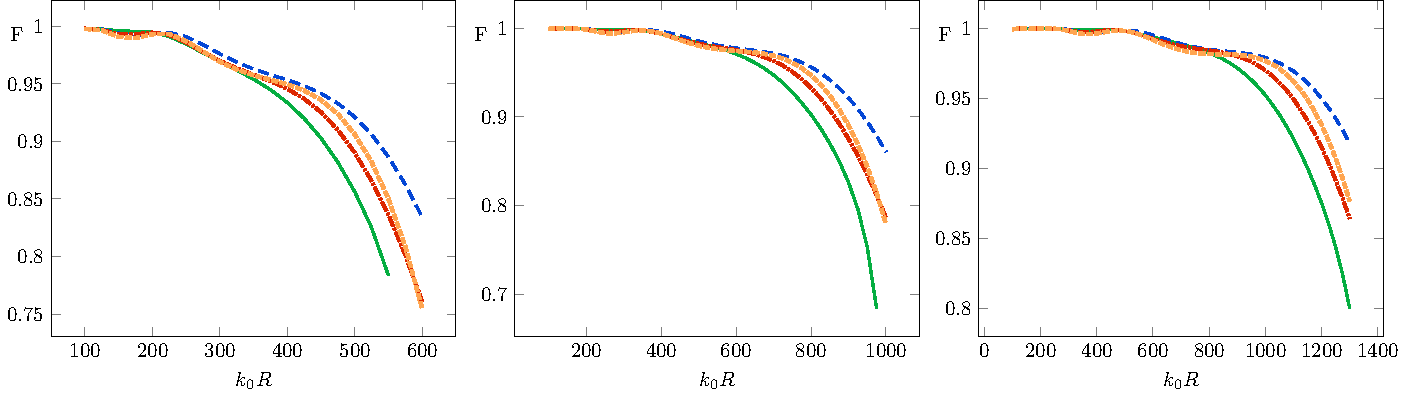
\includegraphics[width = \textwidth]{gfx/fidelities.pdf}
	\caption{Comparison of different fidelities for $ \omega = 3,5,7 $ where the initial momentum $ k_{0} $ varying until a consistent drop in the fidelity was reached. In all the three cases, we can see how the curve obtained for $ n = 2 $ is the one showing the best performances}
	\label{fig:fidelities}
\end{figure*}
Finally, we tested the robustness of each curve for different $ n $ and various speed.
The robustness against dispersion of velocity has been evaluated first by obtaining the curve for a fixed $ k_{0} $ known to ensure the best performances, and then used the same curve to simulate the time evolution of particles with initial velocity included in  $[ k_{0}  -  \epsilon,k_{0}  +  \epsilon]  $ and getting the corresponding fidelity as a function of the inital velocity.
We then defined the robustness as the second derivative of the fidelity with respect to the momentum and repeated this procedure for several $ k_{0} $ and for different $ n $.
The results are summarized in \cref{fig:robustness} and again we can observe that the curve $ \Ga_{2} $ is the one that provides the best performances.
\begin{figure}
	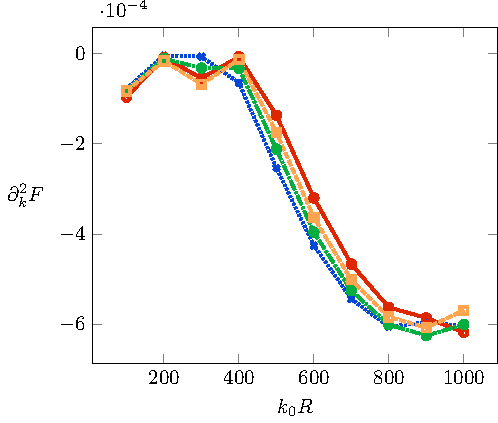
\includegraphics{gfx/robustness.pdf}
	\caption{Plot outlining the robustness for different curves for fixed $ \omega = 7 $ and for different velocities $ k_{0} $. The robustness is defined as the second derivative of the fidelity with respect to the initial momentum and again the best results are obtained for $ n = 2 $ }
	\label{fig:robustness}
\end{figure}
